% Activate the following line by filling in the right side. If for example the name of the root file is Main.tex, write
% "...root = Main.tex" if the chapter file is in the same directory, and "...root = ../Main.tex" if the chapter is in a subdirectory.

%!TEX root =  main.tex

\chapter{Introducción} \label{cha:intro}

\begin{fullwidth}
\textit{En este párrafo, se describe un pequeño resumen del capítulo. \lipsum[1]} \newline
\end{fullwidth}

%\section{Evolución de la Inteligencia Artificial y su Aplicación en Medicina} \label{sec:evol} % cada vez que quiera referenciarme a esta seccion usare la etiqueta \ref{sec:evol} 

%\newthought{Human factor} still has a decisive influence on the evaluation of discontinuities on the radiographic film. An incorrect classification may disapprove a piece in good conditions or approve a piece with discontinuities exceeding the limit established by the applicable standards. The human expert  has as role to inspect each film in order to detect the presence of possible defects which he must then identify and measure. This work is made particularly delicate because of a low size of certain defects, bad contrast and noisy nature of the radiographic film. The human expert often works in cases where its visual system is exposed a extreme conditions and, that is why the subjectivity in the mechanisms of detection and measurement is not negligible. Therefore, a reliable and automatic detection of these heterogeneities in welded joints without human supervision is one of the most important challenges in \gls{NDT} \sidenote[][-6\baselineskip]{Non-destructive testing is the process of inspecting, testing, or evaluating materials, components or assemblies for discontinuities, or differences in characteristics without destroying the serviceability of the part or system. In other words, when the inspection or test is completed the part can still be used.} for \gls{RT} \sidenote[][]{Industrial radiography involves exposing a test object to penetrating radiation so that the radiation passes through the object being inspected and a recording medium placed against the opposite side of that object.  For thinner or less dense materials such as aluminum, electrically generated x-radiation (X-rays) are commonly used, and for thicker or denser materials, gamma radiation is generally used.}. 

%The purpose of the automation of the process of defect detection of digitised radiographs is to reduce time and eliminate the subjective aspect in the analysis realised by the inspector. In this way the reliability in the inspection is enhanced due to the automated evaluation is done by computer programs based on machine learning. The progresses in computer science and artificial intelligence have allowed the defect detection and classification can be carried out by using pattern recognition methods. Therefore, the entire process of detection and classification can be made in an automatic and much more reliable way as it is not a subjective analysis performed by a human expert.

%Classically, automatic defects detection was normally carried out by a well-known pattern recognition techniques \sidenote{Pattern recognition is the ability to detect arrangements of characteristics or data that yield information about a given system or data set. Pattern recognition is closely related to \gls{AI} and \acrfull{ML}.} as image acquisition and  pre-processing, image segmentation, morphological operations, labelling, feature extraction, and classification. After digitising the radiographic film, the pre-processing  stage is devoted to improve the quality of the image in order to better recognise defects (e.g., noise removal, integration ({\color{red}{what integration?}}), contrast enhancement, etc.) The image segmentation stage divides the digital image into disjoint regions with the purpose of separating the parts of interest from the rest of the scene. ({\color{red}{lack labelling stage}}). Subsequently, the feature extraction stage is focused principally around the measurement of invariant attributes deduced from moments and geometric parameters calculation of the \acrfull{RoI}. Finally, the classification stage assigns each segmented region according to the extracted features to pre-established category of weld defect. Typically, in defect detection in welded joints, four categories of defects can be distinguished according to their shape. \begin{enumerate*}[label=\Ordinalstringnum{\arabic*} Flaw:,nosep]\item the shape is lengthened and rectilinear such as cracks and undercuts; \item the shape is lengthened and rectangular as lack of penetration; \item the spherical shape as porosities; and\item the irregular shape (no lengthened and non-spherical) such as solid inclusions and slag inclusions.\end{enumerate*}


%\acrfull{ML} algorithms have been widely used in computer vision applications for decades. The types and subtypes  of machine learning algorithms are shown in Figure \ref{fig:MLAlg}. Supervised learning algorithms build a mathematical model of a set of data that contains both the inputs and the desired outputs. The data is known as training data, and consists of a set of training examples. Each training example has one or more inputs and a desired output, also known as a supervisory signal. In the case of semi-supervised learning algorithms, some of the training examples are missing the desired output. Unsupervised learning algorithms take a set of data that contains only inputs, and find structure in the data, like grouping or clustering of data points. The algorithms therefore learn from test data that has not been labelled, classified or categorised. Instead of responding to feedback, unsupervised learning algorithms identify commonalities in the data and react based on the presence or absence of such commonalities in each new piece of data. Reinforcement learning is an area of machine learning concerned with how software agents ought to take actions in an environment so as to maximise some notion of cumulative reward.
% \begin{figure}[!h]
% % Activate the following line by filling in the right side. If for example the name of the root file is Main.tex, write
% "...root = Main.tex" if the chapter file is in the same directory, and "...root = ../Main.tex" if the chapter is in a subdirectory.
 
%!TEX root =  ../main.tex

 \begin{tikzpicture}
   [small mindmap,
 every node/.style={concept, execute at begin node=\hskip0pt}, 
 root concept/.append style={
 	concept color=red!50, text width=2.2cm}, 
 text=white, 
 grow cyclic, 
 level 1/.append style={text width=1.8cm}, 
 level 2/.append style={text width=1.4cm}
 ] 
 \node [root concept] {\sf \Large Machine Learning} % root 
 child [concept color=blue, grow=north east] { node {\sf \scriptsize Supervised Learning}
       child [concept color=blue!60, grow=north]{ node { \sf \scriptsize Classification} 
 child [concept color=blue!90!black, level distance=1cm, grow=126]{ node [label={[blue!40!black]west:\sf Image Classification},scale=0.3]{ } } 
 child [concept color=blue!90!black, level distance=1cm, grow=54]{ node [label={[blue!40!black]right:\sf Customer Retention},scale=0.3]{ } } 
 child [concept color=blue!90!black, level distance=1cm, grow=198]{ node [label={[blue!40!black,xshift=1.5mm]left:\sf Big Data Visualisation},scale=0.3]{ } } 
 child [concept color=blue!90!black, level distance=1cm, grow=342]{ node [label={[blue!40!black]right:\sf Diagnostics},scale=0.3]{ } }         
       }
        child [concept color=blue!60, grow=south east]{ node { \sf \scriptsize Regression} 
 child [concept color=blue!90!black, level distance=1cm,grow=90]{ node [label={[blue!40!black,yshift=1.5mm]east:\sf \mbox{Advertising Popularity} Prediction},scale=0.3]{ } } 
 child [concept color=blue!90!black, level distance=1cm,grow=270]{ node [label={[blue!40!black,xshift=-1mm]right:\sf Weather Forecasting},scale=0.3]{ } } 
 child [concept color=blue!90!black, level distance=1cm,grow=330]{ node [label={[blue!40!black,xshift=-1mm]east:\sf Market Forecasting},scale=0.3]{ } } 
 child [concept color=blue!90!black, level distance=1cm,grow=30]{ node [label={[blue!40!black, yshift=-1.5mm]right:\sf Extimating Life Expectacting},scale=0.3]{ } } 
  child [concept color=blue!90!black, level distance=1cm, grow=210]{ node [label={[blue!40!black,xshift=1mm]left:\sf Population Growth Prediction},scale=0.3]{ } }          
        }
 } 
 child [concept color=magenta!60!black,  grow=south] { node  {\sf \scriptsize \mbox{Reinforcement} Learning}
       child [concept color=magenta!80!black, level distance=1.25cm, grow=30]{ node [label={[magenta!90!black,xshift=-1.5mm]right:\sf Game AI},scale=0.25]{ } } 
       child [concept color=magenta!80!black, level distance=1.25cm, grow= 330]{ node [label={[magenta!90!black]east:\sf Skill Acquisition},scale=0.25]{ } } 
       child [concept color=magenta!80!black, level distance=1.25cm, grow=270]{ node [label={[magenta!90!black]right:\sf Learning Task},scale=0.25]{ } } 
       child [concept color=magenta!80!black, level distance=1.25cm, grow=210]{ node [label={[magenta!90!black]left:\sf Robot Navigation},scale=0.25]{ } } 
       child [concept color=magenta!80!black, level distance=1.25cm, grow=150]{ node [label={[magenta!90!black,xshift=1mm]left:\sf Real-Time Decisions},scale=0.25]{ } } 
 } 
 child [concept color=green!60!black, grow=north west] { node {\sf \scriptsize Unsupervised Learning} 
   child  [concept color=green!80!black, grow=north] { node { \sf \scriptsize \mbox{Dimensionality} Reduction} 
 child [concept color=green!60!black, level distance=1cm, grow=126]{ node [label={[green!40!black]left:\sf Meaningful Compression},scale=0.3]{ } } 
 child [concept color=green!60!black, level distance=1cm, grow=54]{ node [label={[green!40!black]right:\sf Structure Discovery},scale=0.3]{ } } 
 child [concept color=green!60!black, level distance=1cm, grow=198]{ node [label={[green!40!black]left:\sf Big Data Visualisation},scale=0.3]{ } } 
 child [concept color=green!60!black, level distance=1cm, grow=342]{ node [label={[green!40!black, xshift=-2.5mm]right:\sf Feature Elicitation},scale=0.3]{ } }   
   }
   child  [concept color=green!80!black, grow=south west] { node { \sf \scriptsize Clustering} 
child [concept color=green!60!black, level distance=1cm, grow=north]{ node [label={[green!40!black]left:\sf Recommender System},scale=0.3]{ } } 
child [concept color=green!60!black, level distance=1cm, grow=south west]{ node [label={[green!40!black]left:\sf Targetted Marketing},scale=0.3]{ } } 
 child [concept color=green!60!black, level distance=1cm, grow=south east]{ node [label={[green!40!black]right:\sf Customer Segmentation},scale=0.3]{ } } 
   }
   %... % as before 
   };
 \end{tikzpicture}
% %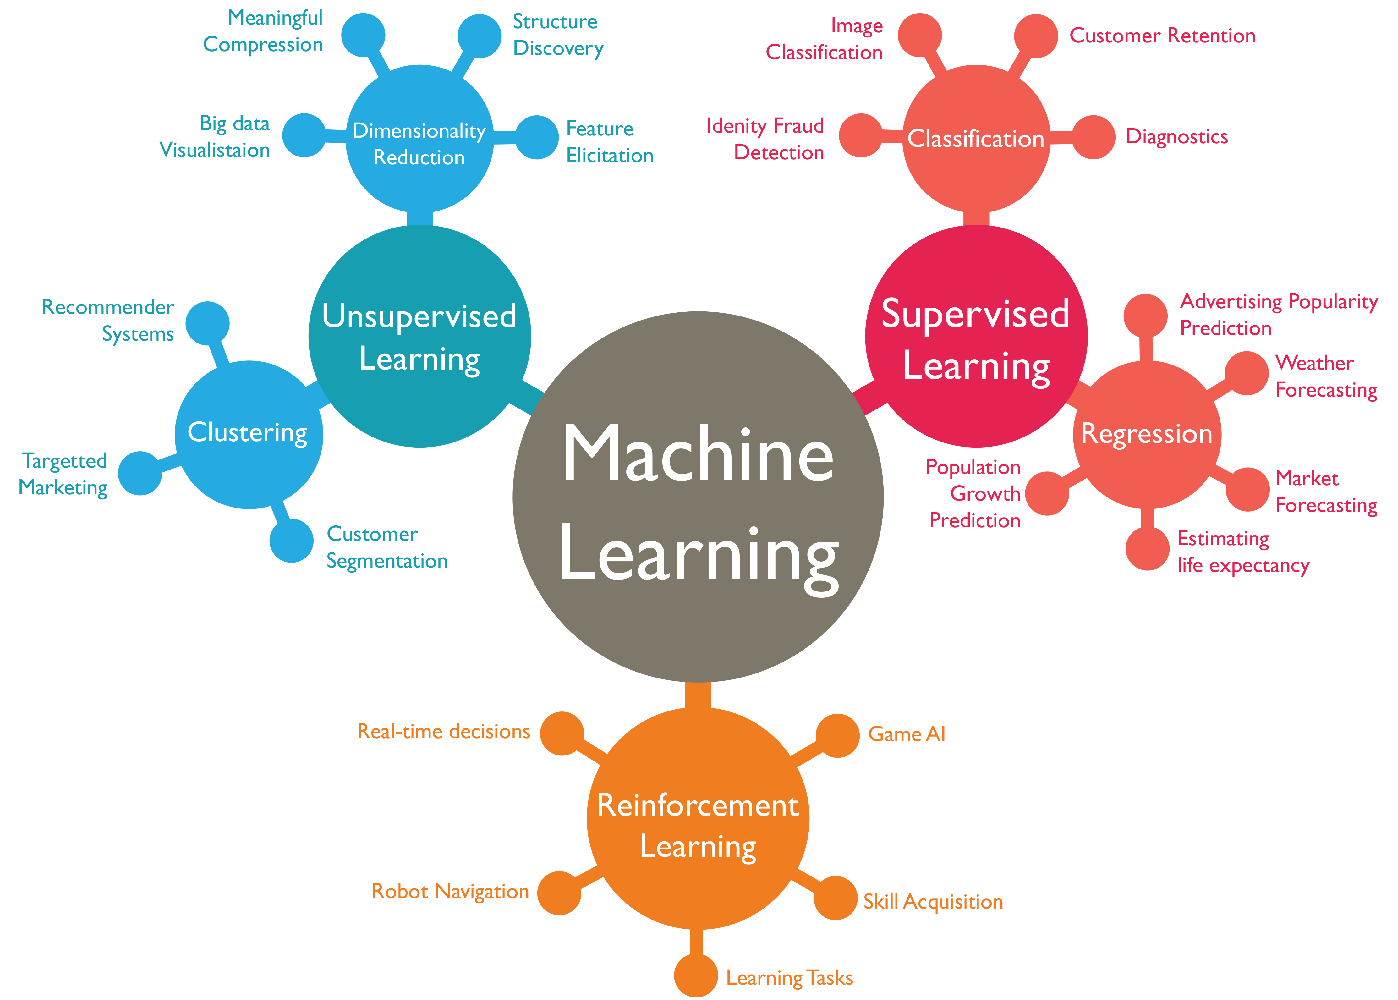
\includegraphics[width=\linewidth]{Introduction/MLAlg.png}
% \caption{The types of \gls{ML} algorithms differ in their approach. Supervised learning, input data is called training data and has a known label or result. A model is prepared through a training process in which it is required to make predictions and is corrected when those predictions are wrong. The training process continues until the model achieves a desired level of accuracy on the training data. Unsupervised learning, input data is not labelled and does not have a known result. A model is prepared by deducing structures present in the input data. This may be to extract general rules. It may be through a mathematical process to systematically reduce redundancy, or it may be to organise data by similarity. Reinforcement learning, Input data is a mixture of labelled and unlabelled examples. There is a desired prediction problem but the model must learn the structures to organise the data as well as make predictions. }
% \label{fig:MLAlg}
% \end{figure}

% \gls{ML} has emerged as a useful tool for modeling problems that are otherwise difficult to formulate exactly. While classical algorithms are explicitly programmed by hand to perform a specific task, with \gls{ML}, some portion of the human contribution is replaced by a learning algorithm. \gls{ML} was becoming more and more practical over the years  because of computational capacity over data was gone increasing. However, everything changed with the appearance of powerful \Glspl{GPU}\sidenote{A \acrfull{GPU} is a very efficient electronic circuit at manipulating computer graphics and image processing. \glspl{GPU} are located on plug-in cards, in a chipset on the motherboard or in the same chip as the \gls{CPU}.}. Modern \glspl{GPU} are very efficient at manipulating computer graphics and image processing. Their highly parallel structure makes them more efficient than general-purpose \acrfullpl{CPU} for algorithms that process large blocks of data in parallel. Nowadays, a new modern subfield of \gls{ML} called Deep Learning is providing a new way in detecting the object automatically.


% Deep learning-based models have had great success in classification by automating both the learning than extracting the features and by using GPUs. Its performance has been demonstrated with large-scale image datasets like ImageNet, which contains more than 10 million images belonging to more than 20 thousand classes. These new deep neural networks like Alexnet, VGG, GoogLeNet and ResNet have shown great performance by reducing the top-1 error. The top-1 error is the rate of error in image classification for 1000 categories. A deep learning model performs classification tasks directly from images, text, or sound.  Deep learning models can achieve cutting edge accuracy, which sometimes exceeds performance at the human level. These neural network architectures are deep because they contain many layers and because they are trained using a large set of labelled data.

% But the problem is that the state-of-the-art models for object detection have not yet been widely applied to radiographic welding image data.  {\color{red}{REMAKE this paragraph AND EXPAND}}

% \section{Related Work}\label{sec:stateofart} 

% Computer scientists around the world have been trying to find ways to make machines extract meaning from visual data for about 60 years now. In the early 1960s, it seemed that a new AI tool was going to make it possible for a machine to be able to learn enough to be able to extract high-level information from huge amounts of data. It was called \acrfull{ANN}. But neural network research stagnated in 1969 after machine learning research by Minsky and Papert\cite{MinskyPapert:69}, who discovered two key issues with the computational machines that processed neural networks. The first was that basic perceptrons were incapable of processing the exclusive-or circuit. The second was that computers didn't have enough processing power to effectively handle the work required by large neural networks. Neural network research slowed until computers achieved far greater processing power.

% However, everything has changed with the appearance of powerful \acrfullpl{GPU}. Now \glspl{GPU} would be able to address more computational cost in the treatment of many input data and many layers of processing. Now, the underlying idea is to trust Big Data\sidenote{Big Data is a field that treats ways to analyze, systematically extract information from, or otherwise deal with data sets that are too large or complex to be dealt with by traditional data-processing application software. } and its accessibility. If a neural network is fed large enough and is multilayer (deep) enough, it is expected that the backpropagation algorithm can adapt the neural weights of the network for its learning.  In a few years only, numerous models of deep neural networks have appeared (naming a few only): MLP: Multi-Layer Perceptron, CNN: Convolutional Neural Network, R-CNN: Region Convolutional Neural Network, RNN: Recurrent Neural Network , BRNN: Bi-directional Recurrent Neural Network, LSTM: Long Short-Term Memory, 3D-CNN: 3D Convolutional Neural Network, GAN: Generative Adversarial Networks, DQN: Deep QNetwork (reinforcement), RBM: Restricted Bolzmann Machine, DBN: Deep Belief Network, and more.


% The convolutional-neural-networks is a subclass of neural-networks which have at least one convolution layer. They are great for capturing local information (eg neighbor pixels in an image or surrounding words in a text) as well as reducing the complexity of the model (faster training, needs fewer samples, reduces the chance of overfitting). \glspl{CNN} can be considered as automatic extractors of the characteristics of the image. If an algorithm based on a vector of pixels is used, a large amount of spatial interaction between the pixels is lost. While a \gls{CNN} effectively uses information from adjacent pixels to reduce the image by convolution layers, for the final use of a prediction and classification layer. Two very important features differentiate them from standard feedforward neural networks. The first feature is that their learning ability can be controlled by varying the depth and breadth of the layers that make up the network. The second feature is that \glspl{CNN} have much fewer connections and parameters than calculating, so they are easier to train even though they are theoretically worse in terms of performance.

% A \gls{CNN}, in specific, has one or more layers of convolution units. A convolution unit receives its input from multiple units from the previous layer which together create a proximity. Therefore, the input units (that form a small neighborhood) share their weights. The convolution units (as well as pooling units) are especially beneficial as:
% \begin{itemize}
% \item They reduce the number of units in the network (since they are many-to-one mappings). This means, there are fewer parameters to learn which reduces the chance of overfitting as the model would be less complex than a fully connected network.
% \item They consider the context/shared information in the small neighborhoods. This future is very important in many applications such as image, video, text, and speech processing/mining as the neighboring inputs (e.g., pixels, frames, words, etc) usually carry related information.
% \end{itemize}



% Currently, main approaches to the classification and detection of objects make use of these new methods of machine learning. In order to improve their performance with respect to the classical methods, it is usual to collect very large data sets, use more powerful learning models and use better techniques to avoid the overfitting of the networks. Until relatively recently, the labelled image datasets were relatively small, approximately tens of thousands of images (e.g., NORB\cite[-26.2\baselineskip]{1315150}, Caltech-101/256\cite[-16\baselineskip]{Fei_Fei_2007}\cite[-8.4\baselineskip]{griffin2007caltech} and CIFAR-10/100\cite[-6\baselineskip]{krizhevsky2009learning}.) The simplest detection and classification tasks can be solved quite well with data sets of this size. But objects in realistic environments show considerable variability, so to learn how to detect them it is necessary to use much larger training sets, but only recently has it been possible to collect data sets labelled with millions of images. The new larger datasets include LabelMe\cite[-6\baselineskip]{Russell_2007}, which consists of hundreds of thousands of fully segmented images, and ImageNet\cite{5206848}, which consists of more than 15 million high resolution labelled images in more than 22,000 categories.


% This concept was first presented by Yann LeCun in 1998 for the classification of digits in MNIST\cite{lecun1998mnist}, where he used a single convolution layer. Later, it was popularized with Alexnet by Alex Krizhevsky  in 2012. Alexnet used several layers of convolution to win ImageNet's Large Scale Visual Recognition Competition (LSVRC)\cite{NIPS2012_4824}  on September 30, 2012. The network made a top-5 error of 15.3\%. more than 10.8 percentage points lower than of the runner-up. The main result of the original article was that the depth of the model was essential for its high performance, which was computationally expensive, but was feasible due to the use of \acrfull{GPU} during training.

% In short, thanks to the powerful current \glspl{GPU} that allow the training of large \glspl{CNN}, combined with a highly optimized implementation of 2D convolution layers, and the recent emergence of data sets, such as ImageNet, which contain enough labeled examples, these deep convolutional neuronal models can be trained  without excessive overfitting.

% \subsection{ A Short History of Deep Learning} 

% Machine learning refers to any technique that focuses on teaching the machine how it can learn statistical parameters from a large amount of training data. One particular type of machine learning is artificial neural networks, which learn a network of nonlinear transformations that can approximate very complicated functions of wide arrays of input variables. Recent advances in artificial neural networks have to do with how to train deep neural networks, which have more layers than normal and also special structure to deal with the challenges of learning more layers. Deep learning is a specific variety of a specific type of machine learning. 

% Most Deep Learning methods deal with the extraction of meaningful information from the contents of digital image or video. This is quite different from simple image processing, which involves manipulating visual information on the pixel level. Applications of computer vision include image classification, visual detection, 3D reconstruction  scenes from 2D images, image recovery, augmented reality, machine vision and traffic automation, the detection of objects, which is our interest.

% One of the most influential articles in Computer Vision was published by two neurophysiologists, David Hubel and Torsten Wiesel\cite[-11\baselineskip]{hubel:single}, in 1959. Its publication described the central response properties of a cat's visual cortical neurons. The researchers established, through their experimentation, that complex neurons exist in the primary visual cortex and that visual processing always begins with simple structures such as oriented edges. This is essentially the basic principle behind deep learning.

% In 1957, Russell Kirsch and his colleagues developed an apparatus  (a digital image scanner) that allowed transforming variations of intensity over the surfaces of images into grids of numbers. One of the first digitally scanned photos, Figure \ref{fig:firstdigitalimage}, was the image of Russell’s infant son. It was just a grainy 5cm by 5cm photo captured as 30,976 pixels (176$\times$176 array), but it has become so incredibly famous that the original image is now stored in the Portland Art Museum.
% \begin{marginfigure}[-30\baselineskip]
% \resizebox{\linewidth}{!}{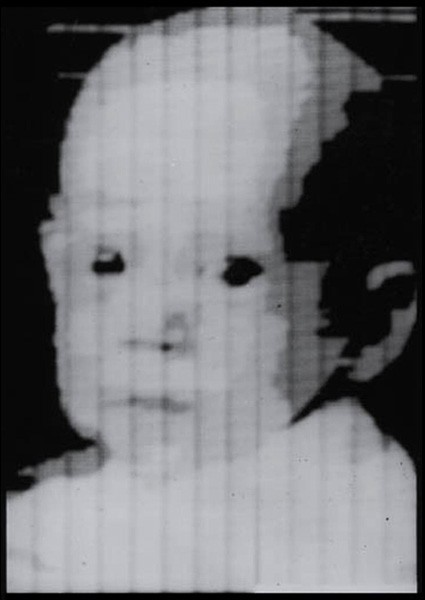
\includegraphics{Introduction/firstscanimage.jpg}}
% \caption{January 01, 1957. Computer pioneer Russell Kirsch and his colleagues created the first digital image of his infant son Walden (\url{https://www.nist.gov/node/774341}) as part of their efforts to develop a way for the \acrfull{SEAC}, a first generation computer designed and built at \acrfull{NIST}, to recognize numbers and letters.}
% \label{fig:firstdigitalimage}
% \end{marginfigure}

%  in 1963, Lawrence Roberts published his Ph.D thesis\cite{roberts1963machine} which is widely considered to be one of the precursors of modern Computer Vision. Roberts described the process of deriving 3D info about solid objects from 2D photographs. He basically reduced the visual world to simple geometric shapes. He affirmed that the processes of 2D to 3D construction, followed by 3D to 2D display, were a good starting point for future research of computer-aided 3D systems. Lawrence didn’t stay in Computer Vision for long. Instead, he went on to join \acrfull{DARPA} and is now known as one of the inventors of the Internet.

% \gls{AI} became an academic discipline in the 1960s. Some of the researchers were so optimistic about the future of the field that they believed it would not take more than 25 years to create a computer as intelligent as a human being. Seymour Papert\cite{article}, professor in the artificial intelligence laboratory at MIT, decided to launch the Summer Vision Project and solve, in a few months, the problem of artificial vision. They tried to design a platform that could automatically perform background/foreground segmentation and extract non-superimposed objects from real-world images. The project wasn’t a success. However, that project was, according to many, the official birth of Computer Vision  as a scientific field.

% In 1982, David Marr, a British neuroscientist, published a paper\cite{Marr:1982:VCI:1095712} on Hubel and Wiesel's ideas of how the brain processes information and how vision processing does not begin by determining holistic objects, that is, as a whole, but rather through the parts that compose them. Marr established that the vision is hierarchical. He argued that the main function of the vision system is to create 3D representations of the environment so that we can interact with it. He introduced a framework for vision where low-level algorithms are used that detect edges, curves, corners, etc., as steps towards a high-level understanding of visual data. David Marr’s work was groundbreaking at the time, but it was very abstract and high-level. It didn’t contain any information about the kinds of mathematical modeling that could be used in an artificial visual system, nor mentioned any type of a learning process.

% Almost at the same time, a Japanese computer scientist, Kunihiko Fukushima, also deeply inspired by Hubel and Wiesel, built a self-organized artificial network of simple and complex cells that could recognize patterns and that was not affected by their position changes. The network, called Neocognitron\cite{fukushima1980neocognitron}, included several convolutional layers whose receptive fields (typically rectangular) had weight vectors (known as filters). The function of these filters was to slip through 2D arrays of input values (like the pixels of a digital image) and, after performing several calculations, to produce activation events (2D arrays) that would be used as inputs for subsequent layers of the net. The Neocognitron of Fukushima is possibly the first neural network that deserves the nickname of "deep". He is the first ancestor of today's \glspl{CNN}.

% A few years later, in 1989, a young French scientist Yann LeCun applied a backpropagation style learning algorithm to the architecture of the convolutional neural network of Fukushima. After working on the project for some years, LeCun launched LeNet-5\cite[-8\baselineskip]{lecun-89}, the first modern CNN that introduced some of the essential ingredients that we still use in CNNs today, as is shown in Figure\ref{fig:lenet5}. Like Fukushima before him, LeCun decided to apply his invention to character recognition and even launched a commercial product to read zip codes\cite[-6\baselineskip]{lecun1989backpropagation}. In addition, his work resulted in the creation of the MNIST\cite{lecun1998mnist} data set of handwritten digits, perhaps the most famous reference data set in machine learning.
% \begin{figure}[!htbp]
% \begin{center}
% \resizebox{\linewidth}{!}{%\noindent\begin{minipage}[c]{\linewidth}\centering
% \vspace{\baselineskip} \small 
%\mtotex{g}{quick60}
%1 row


\newcommand{\xangle}{0}
\newcommand{\yangle}{90}
\newcommand{\zangle}{220}

\newcommand{\xlength}{1}
\newcommand{\ylength}{1}
\newcommand{\zlength}{0.9}

\pgfmathsetmacro{\xx}{\xlength*cos(\xangle)}
\pgfmathsetmacro{\xy}{\xlength*sin(\xangle)}
\pgfmathsetmacro{\yx}{\ylength*cos(\yangle)}
\pgfmathsetmacro{\yy}{\ylength*sin(\yangle)}
\pgfmathsetmacro{\zx}{\zlength*cos(\zangle)}
\pgfmathsetmacro{\zy}{\zlength*sin(\zangle)}

%\def\space{.5} %space betwwen layer
%(0,0,0) coordinate (O);
 \begin{tikzpicture}
[   x={(\xx ,\xy )},
    y={(\yx ,\yy )},
    z={(\zx ,\zy )},
]
 
\newcommand{\networkLayer}[9]{
			\def\H{#1}% Height Y
			\def\W{#2}% Width XZ
			\def\D{#3} % Depth X
			\def\h{#4} % Height  Filter y 				
			\def\w{#5} % Width XZ Filter
			\def\s{#6} % s distance to next layer 
			\def\oh{#7}% N=1 or S=-1
			\def\ow{#8} %E=1 or W=-1
			\networkLayercontinued#9
			%\def\S1{#8} %
			%\def\S2{#9} %
			%\def\S3{#10} %
			% Draw the layer body.
}			
%NNSVG node[midway,below]{\tiny #3}  node[midway,right,xshift=-2]{\tiny #1}  node[midway,right]{\tiny #2} Tensor opacity Filter opacity Spacing between layers 

\newcommand{\networkLayercontinued}[6]{
% %Filter lateral face  
%\filldraw[opacity=0.8,fill=black!30] (.5*\w,-.5*\h,.5*\w) --++ (0,\h,0)  --++ (-\w,0,-\w) --++ (0,-\h,0) -- (.5*\w,-.5*\h,.5*\w);
%
%%Filter Front Face 
%  \filldraw[opacity=0.8,fill=black!30] (.5*\w,-.5*\h,.5*\w) --++ ( \D,0,0) --++ (0,\h,0) --++  ( -\D,0,0) --++   (0,-\h,0)node[opacity=1,midway,right]{\tiny #4} ;
%  
% %Filter Top Face 
%  \filldraw[opacity=0.8,fill=black!30] (.5*\w,.5*\h,.5*\w) --++ (-\w,0,-\w)node[opacity=1,midway,right]{\tiny #5}  --++ ( \D,0,0)  --++ (\w,0,\w)  --++ ( -\D,0,0); 
%
% \coordinate (A) at (+\D+.5*\w,-.5*\h,.5*\w);
% \coordinate (B) at (+\D+.5*\w,-.5*\h+\h,.5*\w);
% \coordinate (C) at (+\D+.5*\w-\w,-.5*\h+\h,.5*\w-\w);
% \coordinate (D) at (\D+\s,0,0);
% \draw (A) -- (D);
% \draw (B) -- (D);
% \draw (C) -- (D);

% Filter lateral face  
\filldraw[opacity=0.8,fill=black!20] (.25*\ow*\W+0.5*\w,\oh*.25*\H-0.5*\h,.25*\ow*\W+0.5*\w) --++ (0,\h,0)  --++ (-\w,0,-\w) --++ (0,-\h,0) -- (.25*\ow*\W+0.5*\w,\oh*.25*\H-0.5*\h,.25*\ow*\W+0.5*\w);

%Filter Front Face 
  \filldraw[opacity=0.8,fill=black!20] (.25*\ow*\W+0.5*\w,\oh*.25*\H-0.5*\h,.25*\ow*\W+0.5*\w) --++ ( \D,0,0) --++ (0,\h,0) --++  ( -\D,0,0) --++   (0,-\h,0)node[opacity=1,midway,right]{\tiny #4} ;
  
%Filter Top Face 
  \filldraw[opacity=0.8,fill=black!20] (.25*\ow*\W+0.5*\w,\oh*.25*\H-0.5*\h+\h,.25*\ow*\W+0.5*\w) --++ (-\w,0,-\w)node[opacity=1,midway,right]{\tiny #5}  --++ ( \D,0,0)  --++ (\w,0,\w)  --++ ( -\D,0,0); 
\coordinate (A) at (\D+.25*\ow*\W+0.5*\w,\oh*.25*\H-0.5*\h,.25*\ow*\W+0.5*\w);
 \coordinate (B) at (\D+.25*\ow*\W+0.5*\w,\oh*.25*\H-0.5*\h+\h,.25*\ow*\W+0.5*\w);
 \coordinate (C) at (\D+.25*\ow*\W+0.5*\w-\w,\oh*.25*\H-0.5*\h+\h,.25*\ow*\W+0.5*\w-\w);
 \coordinate (D) at (\D+.25*\ow*\W+0.5*\w+\s -.5*\w,\oh*.25*\H-0.5*\h,.25*\ow*\W+0.5*\w-.5*\w);
 \draw[densely dotted] (A) -- (D);
 \draw[densely dotted] (B) -- (D);
 \draw[densely dotted] (C) -- (D);
%(0,0,0) coordinate (o);

%Lateral Face
  \filldraw[opacity=0.5,fill=black!20] (.5*\W,-.5*\H,.5*\W) --++ (0,\H,0)  --++ (-\W,0,-\W) --++ (0,-\H,0) -- (.5*\W,-.5*\H,.5*\W);
 %Front Face 
  \filldraw[opacity=0.5,fill=black!20] (.5*\W,-.5*\H,.5*\W) --++ ( \D,0,0)node[opacity=1,midway,below,label=below:\tiny #6]{\tiny #3} --++ (0,\H,0) --++  ( -\D,0,0) --++   (0,-\H,0)node[opacity=1,midway,right]{\tiny #1} ;
  %Top Face 
  \filldraw[opacity=0.5,fill=black!20] (.5*\W,.5*\H,.5*\W) --++ (-\W,0,-\W)node[opacity=1,midway,right]{\tiny #2}  --++ ( \D,0,0)  --++ (\W,0,\W)  --++ ( -\D,0,0);



\tikzset{shift={(\D+\s,0,0)}};

}
% From left to right
% 1 Height Y, 2 Width XZ, 3 Depth X, 4 Height  Filter y, 5 Width XZ Filter, 6 s distance to next layer,7 N=1 or S=-1,8 E=1 or W=-1,  9 text H, 10 text W, 11 Text depth, 12 text w filter, 13 text height filter ,14 type of layer

\networkLayer{3.2}{3.2}{0.1}{0}{0}{1}{0}{0}{{32}{32}{1}{}{}{Image}}
\networkLayer{2.8}{2.8}{0.6}{0.5}{0.5}{0.8}{1}{-1}{{23}{23}{5}{5}{5}{Conv}}
\networkLayer{1.4}{1.4}{0.6}{0.2}{0.2}{0.5}{1}{-1}{{14}{14}{6}{2}{2}{Av. Pool}}
\networkLayer{1}{1}{1.6}{0.5}{0.5}{0.3}{1}{1}{{10}{10}{16}{5}{5}{Conv}}
\networkLayer{0.5}{0.5}{1.6}{0}{0}{0.3}{1}{1}{{5}{5}{16}{}{}{Av. Pool}}
\networkLayer{6.0}{0.1}{0.1}{0}{0}{1}{0}{0}{{120}{1}{1}{}{}{Fully Conn}}
\networkLayer{4.2}{0.1}{0.1}{0}{0}{1}{0}{0}{{84}{1}{1}{}{}{Fully Conn}}
\networkLayer{1}{0.1}{0.1}{0}{0}{0}{0}{0}{{10}{1}{1}{}{}{0-9 digits}}
%\networkLayer{5}{0.1}{0.01}{0}{0}{1}{0}{0}{{50}{1}{1}{}{}{}}
%\networkLayer{5}{0.1}{0.01}{0}{0}{1}{0}{0}{{50}{1}{1}{}{}{}}
%\networkLayer{5}{0.1}{0.01}{0}{0}{0}{0}{0}{{50}{1}{1}{}{}{}}



\end{tikzpicture}

%\captionof{figure}{.}
%\label{Symbolic_label52}
%\end{minipage}
}
% \caption{Yann LeCun, Leon Bottou, Yosuha Bengio and Patrick Haffner proposed a neural network architecture for handwritten and machine-printed character recognition in 1990’s which they called LeNet-5. The architecture is straightforward and simple to understand that’s why it is mostly used as a first step for teaching Convolutional Neural Network. The LeNet-5 architecture consists of two sets of convolutional and average pooling layers, followed by a flattening convolutional layer, then two fully-connected layers and finally a softmax classifier.}
% \label{fig:lenet5}
% \end{center}
% \end{figure}


% In the late 1990s and early 2000s, many researchers stopped trying to reconstruct objects by creating 3D models of them (the path proposed by Marr) and instead directed their efforts towards recognizing objects based on characteristics. David Lowe's paper\cite{Lowe:04} describes a visual recognition system that uses local characteristics that are invariant to rotation, location and, partially, to changes in lighting. These characteristics, according to Lowe, are somewhat similar to the properties of the neurons that are found in the lower temporal cortex and are involved in the processes of object detection in the primate vision.

% During those years, the first algorithm of detection of faces that worked in real time was presented by Paul Viola and Michael Jones\cite{viola2001rapid}. Although it was not based on deep learning, the algorithm had a certain flavor to deep learning. It learned which characteristics (very simple, Haar-like features\cite{haar1910theorie}) could help to locate faces when it processed the images,. Today, the Viola/Jones facial detector is still widely used. It is a strong binary classifier built from several weak classifiers. During the learning phase, which is the part that consumes the most time, the cascade of weak classifiers is trained using Adaboost\cite{schapire1999improved}. To find the object of interest (face), the input image is partitioned into rectangular patches that are sent to the cascade of weak detectors. If a patch manages to pass through each stage of the cascade, it is classified as positive, if not, the algorithm rejects the patch immediately. This process is repeated many times in several scales. Five years after the article was published, Fujitsu launched a camera with a real-time face detection function based on the Viola/Jones algorithm.

% As the field of computer vision progressed, the community felt a strong need for a benchmark image dataset and standard evaluation metrics to compare the performance of models. In 2005, the Pascal VOC project\cite{everingham20052005} was launched, which provided a standardized data set for the classification of objects, as well as a set of tools to access the data set and annotations. The founders also held an annual competition, from 2006 to 2012, which allowed evaluating the performance of different methods for the recognition of the object classes.

% In 2009, another important feature-based model was developed by Pedro Felzenszwalb, David McAllester and Deva Ramanan\cite{4587597}, the deformable part model. Basically, the model decomposes the objects into collections of parts (based on pictorial models introduced by Fischler and Elschlager\cite{1672195} in the 1970s), imposes a set of geometric constraints between them and models the centers of potential objects that were taken as latent variables. The model showed great performance in object detection tasks (where bounding boxes were used to locate objects) and outperformed template matching and other object detection methods that were popular at the time.

% In 2010, ImageNet's Large-Scale Visual Recognition Competition (ILSVRC) started. As PASCAL VOC is done annually and includes a post-competition workshop where participants discuss what they have learned and what the most innovative models have been in the challenge. But unlike Pascal VOC, which only had 20 categories of objects, the ImageNet data set contains more than one million images, which are cleaned manually, in 1k of object classes. Since its inception, the ImageNet challenge has become a point of reference in the object category classification and in object detection in a large number of categories. In 2010 and 2011, the ILSVRC error rate in image classification was around 26\%. But in 2012, a team from the University of Toronto put a convolutional neural network model (AlexNet) to compete and that changed everything. The model, similar in its architecture to the LeNet-5 of Yann LeCun, achieved an error rate of 16.4\%. This was a turning point for CNN.

% \subsection{Welding Defect Detection and Classification}
% In the last three decades, there is a increasing requirement in the quality of equipments in the industry. Radiographic testing is one of the oldest non-destructive testing and therefore is commonly used in the detection of welded joints quality in many industrial fields such as the nuclear, chemical and aeronautical. The real-time detection and automatic identification for welding defects from the digitised images become in a focus of \gls{NDT} research. For long time, several efforts have been devoted to the development of such a system which can detect and classify the welding defects automatically using X-ray digitised images.

% D. Mery\cite[-5\baselineskip]{Mery_2003} proposed a scheme for detecting weld defects from digitised film images based on three main steps: segmentation, texture features extraction and classification. The higher precision of the system achieved 90.91\%. Silva et al.\cite[-2\baselineskip]{da_Silva_2004} described a non-linear classifier based on \acrfull{ANN} and was compared with the linear classifiers. \acrfull{ANN} or connectionist systems are computing systems vaguely inspired by the biological neural networks that constitute animal brains. An very easy examle of \gls{ANN} is shown in Figure \ref{fig:ann}. The neural network itself is not an algorithm, but rather a framework for many different  \acrfull{ML} algorithms to work together and process complex data inputs. Such systems "learn" to perform tasks by considering examples, generally without being programmed with any task-specific rules. %
% \begin{figure}[!htbp]
% \centering
% \resizebox{\linewidth}{!}{\input{Introduction/ann}}
% \caption{Each circular node represents an artificial neuron and an arrow represents a connection from the output of one artificial neuron to the input of another. Typically, artificial neurons are aggregated into layers. Different layers may perform different kinds of transformations on their inputs. Signals travel from the first layer (the input layer), to the last layer (the output layer), possibly after traversing the layers multiple times.}
% \label{fig:ann}
% \end{figure}

% J. Kumar et al.\cite[-3\baselineskip]{Kumar_2014} extracted the texture features in different direction for several spatial pixel distances for classifying the different flaws and obtained an overall classification accuracy of 86.1\% by using \gls{ANN}.  Vilar et al.\cite{Vilar_2009}propose to use an artificial neural network (ANN) for weld defect classification where three different methods for improving network generalisation was used. Zapata et al.\cite{Zapata_2010}   describe an \acrfull{ANFIS} to recognise welding defects in radiographic images using twelve features (geopmetric features) of welding defects which was input data to the \gls{ANFIS} sistem

% The idea underlying in attempting to approach the classification process by means of an \gls{ANN}  is to try that the neural network inputs were as small as possible so that the learning process was admissible in computational cost and therefore in time. Everything changed with the \glspl{GPU},  new backpropagation algorithms and big labelled datasets. Deep Learning has been successfully used in image analysis and automatic object recognition. However, there is not much research that attempts to solve the problem of the recognition of defects in industrial welding through deep learning techniques. Faghih-Roohi et al.\cite[-4\baselineskip]{7727522} propose a deep convolutional neural network solution to the analysis of image data for the detection of rail surface defects as a viable technique for feature learning.  They compare the results of different network architectures characterized by different sizes and activation functions. In this way, they explore the efficiency of the proposed deep convolutional neural network for detection and classification. Yang et al.\cite[-2\baselineskip]{Yang_2018} proposed the technique based on LeNet-5, using improved convolutional neural network to classify X-ray weld images, to detect weld defection. By improving the convolution kernel and the activation function, the accuracy of the classification is improved. The approach based on the CNN-X-ray is more accurate than LeNet-5, \glspl{ANN} and \glspl{SVM}\cite{Shao_2011}\cite{Wang_2014}, with accuracy 99.5\%. Liu et al.\cite{Liu_2018} proposed a VGG16 based weld defect images classification method. By using fully convolutional structure, though they must train the network using the same size input considering of the parallel processing, the defect images used for test can be variable size. This network achieves a testing accuracy on 3000 test images which is large enough compared to others methods. 


% Hou et al.\cite{Hou_2018}  propose a \gls{DCNN} to classify weld defects. The performance of the system was compared using different methods in order to extract deep features from image. To validate the effectiveness of deep features, we cropped patches from the X-ray images as the learning dataset. The best results were obtained for the deep features from the proposed DCNN model, achieving an accuracy of 97.2\%, which is considerably higher than that obtained using the traditional feature extraction methods. 

% Deep Learning has good performance for learning more representative hierarchical features that are more sensitive to classification. But, there is not a large data set of labelled welding images that allows an effective training of these Deep Learning models. The only dataset of welding image is given by Mery et al.\cite{Mery_2015}. This new dataset consisting of 19,407 X-ray images. The images are organized in a public database called GDXray that can be used free of charge, but for research and educational purposes only. The database includes five groups of X-ray images: castings, welds, baggage, natural objects and settings. Each group has several series, and each series several X-ray images. Most of the series are annotated or labeled but not all the images. In such cases, the coordinates of the bounding boxes of the objects of interest or the labels of the images are available in standard text files.

% %Therefore, object detection is one of the classical problems of computer vision and is often described as a difficult task. The difference between objects detection and  classification algorithms is that, in the object detection algorithms, an attempt is made to draw a bounding box around the object of interest to locate it within the image. In addition, it is possible that not necessarily only a bounding box will be drawn. In a case of detection of several objects, there may be many bounding boxes that represent different objects of interest within the image and it does not know how many in advance.%During the 2000s, popular solutions for object detection utilized feature descriptors, such as scale-invariant feature transform (SIFT) [14] developed by David Lowe in 1999 and histogram of oriented gradients (HOG) [15] popularized in 2005. In the 2010s, there has been a shift towards utilizing convolutional neural networks [12] [16] [17].
% %Before the widescale adoption of CNNs, there were two competing solutions for generating bounding boxes. In the first solution, a dense set of region proposals is generated and then most of these are rejected [18]. This typically involves a sliding window detector. In the second solution, a sparse set of bounding boxes is generated using a region proposal method, such as Selective Search [11]. 
% %
% %Combining sparse region proposals with convolutional neural networks has provided good results and is currently popular. 
% %


% %The receptive field\cite{hubel:single}, the biological function which inspired to \gls{CNN}, can be approximated in computers using the convolution operation\cite{Fukushima:1979neocognitron}. The size of the receptive field is adjusted by the size of the convolution mask. In the case of neural networks, the output matrix is also called a feature map, or an activation map after computing the activation function.
% %
% %
% %
% %
% %
% %Due to the number of occurrences of the objects of interest is not fixed, the length of the output layer is variable ---not constant, and therefore it cannot proceed with this problem by building a standard convolutional network followed by a fully connected layer.
% %
% % Copied from Faster R-CNN: Towards Real-Time Object Detection with Region Proposal Networks
% %State-of-the-art object detection networks depend on region proposal algorithms to hypothesize object locations. Advances like SPPnet [1] and Fast R-CNN [2] have reduced the running time of these detection networks, exposing region proposal computation as a bottleneck. Faster RCNN [17] is one of the advanced method of object detection and have a great resolution in the last years.
% %With the great success of the Deep Learning based methods on object detection, several works based on CNN have been designed. In [19] micro-organisms like malaria parasites which are still studied by expert manual inspection and hand counting. This type of object detection task is challenging due to factors like variations in cell shape, density, and color, and uncertainty of some cell classes. They use Faster Region-based Convolutional Neural Network (Faster R- CNN), pre-trained on ImageNet but fine tune with their data, and compare it to a baseline, which is based on a traditional approach consisting of cell segmentation, extraction of several single- cell features, and classification using random forests and they demonstrate that Faster R-CNN outperforms the baseline. Other work [20] made for scale mammography databases enable researchers to evaluate advanced tumor detections applying deep convolution networks (DCN) to mammography images which is one of the common used imaging modalities for early breast cancer. The performance of tumor detection has been developed by a great extent, especially using R-CNNs or Region convolution neural networks. This study evaluates the performance of a simple faster R-CNN detector for mammography lesion detection using a MIAS databases.
% %In this work, we introduce a Region Proposal Network (RPN) that shares full-image convolutional features with the detection network, thus enabling nearly cost-free region proposals. An RPN is a fully convolutional network that simultaneously predicts object bounds and objectness scores at each position. The RPN is trained end-to-end to generate high-quality region proposals, which are used by Fast R-CNN for detection. We further merge RPN and Fast R-CNN into a single network by sharing their convolutional features using the recently popular terminology of neural networks with “attention” mechanisms, the RPN component tells the unified network where to look. Faster R-CNN and RPN are the foundations of the 1st-place winning entries in several tracks that is why it is our advanced method for object detection.


% \section{Structure of Work}\label{sec:struc}
% Since object detection is a combination of several fields of computer vision, we need to discuss several theoretical topics that can seem disparate at first. The structure of this works is as follows. In first chapter, we begin with a short introduction to machine learning and neural networks. Next, we discuss computer vision and object detection as its subfield. We end the chapter by introducing convolutional neural networks as a combination of machine learning and computer vision. In second chapter, we discuss how convolutional networks can be used for object detection, review the relevant literature and methods and our method of Implementation (Faster RCNN).
% In the next chapter, we move to the experimental part. We discuss what kind of experimental setup we used for testing a convolutional network. We discuss not only the details of the experiments, but also the details of the datasets. Further, we discuss how we will evaluate the results.
% we discuss also the practical implementation of the experiments by discussing the required software and hardware and how these were used. We evaluate the results. We provide not only the numerical results, but also some analysis of them. However, the classification of weld defects with convolutional network is left to the last chapter, where we discuss the two implemented methods. We base this discussion on the results of our experiments as well as topics known from the literature. Finally, we provide a review of the work and some concluding remarks.




\section{Evolución de la Inteligencia Artificial y su Aplicación en Medicina} \label{sec:evol} % cada vez que quiera referenciarme a esta seccion usare la etiqueta \ref{sec:evol} 

\newthought{La} \emph{inteligencia artificial} (IA)\sidenote{La inteligencia artificial es un campo de la informática que se enfoca en la creación de sistemas y máquinas capaces de realizar tareas que normalmente requieren inteligencia humana. Estas tareas incluyen el aprendizaje, la percepción, el razonamiento, la toma de decisiones, el reconocimiento de patrones, el procesamiento del lenguaje natural y la resolución de problemas. } ha estado experimentando un crecimiento exponencial en las últimas décadas, se ha consolidado como una de las tecnologías más importantes en muchos campos, de entre ellos, la medicina. Desde sus primeras menciones en la década de 1950 con los trabajos pioneros de Alan Turing en el concepto de máquinas inteligentes y John McCarthy, quien acuñó el término inteligencia artificial en 1956~\cite{mccarthy1956ai}, la IA ha evolucionado significativamente. Inicialmente la mayoría de los avances en IA se basaban en sistemas expertos y en programas con reglas fijas, es decir, sistemas que seguían instrucciones muy concretas, escritas directamente por personas expertas. Estos sistemas eran útiles para tareas específicas, pero eran rígidos y no podían adaptarse a situaciones nuevas, proporcionando soluciones limitadas y altamente dependientes del conocimiento humano explícito. Sin embargo, con la llegada del aprendizaje automático (\emph{Machine Learning, ML}\sidenote{Machine Learning es una rama de la inteligencia artificial que permite a las computadoras aprender patrones y tomar decisiones a partir de datos, sin ser programadas explícitamente para cada tarea.} en las décadas de 1980 y 1990, se inició una transición hacia modelos capaces de aprender patrones a partir de grandes volúmenes de datos, mejorando su capacidad de generalización y adaptabilidad. En la actualidad, el aprendizaje profundo (\emph{Deep Learning, DL})\sidenote{Deep Learning es una subárea del machine learning que utiliza redes neuronales artificiales con múltiples capas para aprender representaciones complejas de datos. Es especialmente efectivo en tareas como reconocimiento de imágenes, procesamiento de lenguaje natural y predicciones avanzadas.} ha revolucionado la IA, permitiendo a los modelos aprender representaciones jerárquicas de los datos, lo que ha llevado a un aumento significativo en el rendimiento de los sistemas de IA en una amplia variedad de tareas, incluyendo la visión por computadora, el procesamiento del lenguaje natural y la robótica.

En el campo de la medicina, la IA ha demostrado ser una herramienta valiosa para el diagnóstico y tratamiento de enfermedades. En particular, la visión por computadora ha sido ampliamente utilizada para el análisis de imágenes médicas, como radiografías (RX)\sidenote{Las radiografías utilizan rayos X para crear imágenes de estructuras internas del cuerpo, especialmente huesos. Los rayos X atraviesan el cuerpo y son absorbidos en diferentes cantidades por los tejidos, creando una imagen en blanco y negro.}, tomografías computarizadas (TC)\sidenote{La tomografía computarizada combina múltiples imágenes de rayos X tomadas desde diferentes ángulos para crear imágenes detalladas en cortes transversales (axiales) del cuerpo. A menudo se usa un medio de contraste para mejorar la visibilidad de ciertos tejidos.} y resonancias magnéticas (RM)\sidenote{La resonancia magnética utiliza campos magnéticos y ondas de radio para generar imágenes detalladas de los tejidos blandos, órganos y estructuras internas. No utiliza radiación ionizante.}. La detección y clasificación de enfermedades a partir de imágenes médicas es una tarea compleja que requiere una gran cantidad de conocimientos y experiencia. Los radiólogos, por ejemplo, deben examinar cuidadosamente las imágenes para identificar patrones y anomalías que puedan indicar la presencia de enfermedades. Sin embargo, este proceso es lento y propenso a errores, ya que los radiólogos pueden pasar por alto detalles importantes o malinterpretar los resultados. La IA puede ayudar a superar estos desafíos, ya que los modelos de aprendizaje profundo pueden aprender a detectar patrones sutiles en las imágenes que pueden ser difíciles de detectar para los humanos. Además, los modelos de IA pueden analizar grandes volúmenes de datos en poco tiempo, lo que puede acelerar el proceso de diagnóstico y tratamiento.

El avance más significativo se produjo con la introducción del aprendizaje profundo (Deep Learning), impulsado por tres factores:
\begin{enumerate}
    \item El incremento en la capacidad de cómputo, especialmente con las unidades de procesamiento gráfico (GPUs), que han permitido entrenar modelos más complejos en tiempos reducidos [3].
    \item La enorme cantidad de datos disponibles hoy en día, gracias a internet, redes sociales, sensores y todo tipo de dispositivos conectados, lo que ha dado a los modelos muchísimo material para aprender y mejorar [4].
    \item Las constantes mejoras en los algoritmos y en las estructuras de las redes neuronales, que han hecho que estos modelos no solo sean más precisos, sino también más capaces de adaptarse a situaciones nuevas y resolver problemas cada vez más complejos [5].
\end{enumerate}

En el campo de la medicina, la IA ha transformado por completo la forma en la que se aborda el diagnóstico, el tratamiento e incluso la investigación. Uno de los ámbitos donde más impacto ha tenido la IA es en el análisis de imágenes médicas , donde las redes neuronales convolucionales (CNNs)\sidenote{CNN (Convolutional Neural Networks, Redes Neuronales Convolucionales) son un tipo de red neuronal profunda diseñada específicamente para procesar datos estructurados en forma de cuadrícula, como imágenes.}  han demostrado ser muy eficaces. Utilizan capas convolucionales para extraer características locales y jerárquicas, lo que las hace muy efectivas en tareas de visión por computadora, como clasificación de imágenes, detección de objetos y segmentación. Este tipo de redes son capaces de analizar imágenes médicas de forma automática, además de realizar tareas de detección, clasificación y segmentación de estructuras anatómicas con niveles de exactitud y precisión similares a los de especialistas humanos en determinadas aplicaciones [6].

Algunos modelos de aprendizaje automático han sido implementados en la identificación temprana de patologías como el cáncer, la retinopatía diabética y enfermedades neurodegenerativas, mejorando así las tasas de detección precoz. Además, la integración de la IA con sistemas de historial clínico permite proporcionar recomendaciones terapéuticas basadas en datos de pacientes, optimizando la toma de decisiones y reduciendo errores médicos. La capacidad de estos sistemas para analizar grandes volúmenes de información ha facilitado la identificación de patrones en datos genómicos y moleculares, impulsando avances en la medicina personalizada y el descubrimiento de nuevos fármacos.

La capacidad de los algoritmos para identificar patrones invisibles al ojo humano ha revolucionado la radiología y otras disciplinas médicas, permitiendo diagnósticos más precisos y la detección temprana de patologías [7]. Tecnologías como U-Net [8], nnU-Net [9] y Transformers en visión médica [10] han mejorado la segmentación automática de tejidos y órganos, mientras que otros modelos basados en redes profundas han permitido la clasificación automática de imágenes en modalidades como radiografías (RX), tomografías computarizadas (TC) y resonancias magnéticas (RM).

Además, la integración de la IA en el ámbito clínico ha abierto nuevas posibilidades en la planificación quirúrgica personalizada, permitiendo a los cirujanos acceder a reconstrucciones tridimensionales precisas de la anatomía del paciente. Estos avances han mejorado la seguridad y la eficiencia de los procedimientos quirúrgicos, reduciendo el margen de error y optimizando la preparación preoperatoria [11].

A pesar de los logros alcanzados, persisten desafíos importantes en la implementación clínica de la IA, incluyendo la necesidad de bases de datos de alta calidad, la validación regulatoria de los modelos y la interpretabilidad de los resultados [12]. El presente trabajo busca abordar estos desafíos mediante el desarrollo de una herramienta basada en IA para la clasificación y segmentación automatizada de imágenes de RM en pacientes oncológicos, con el fin de mejorar la precisión diagnóstica y optimizar la planificación quirúrgica.
        
\section{Principios de las Imágenes Médicas y la Resonancia Magnética} \label{sec:principios}
\subsection{Imágenes Médicas}

Las imágenes médicas desempeñan un papel fundamental en la práctica clínica y la investigación biomédica, permitiendo la evaluación no invasiva de la anatomía y fisiología del cuerpo humano. Existen diversas modalidades de adquisición de imágenes médicas, cada una con aplicaciones específicas según el tipo de tejido o patología a evaluar. Entre las principales técnicas se encuentran:
    \begin{itemize}
        \item Radiografía (RX): Basada en la atenuación diferencial de los rayos X, es ampliamente utilizada para el diagnóstico de fracturas óseas y patologías pulmonares [13].
        \item Tomografía Computarizada (TC): Emplea múltiples proyecciones de rayos X para generar imágenes seccionales del cuerpo, permitiendo una mejor caracterización de estructuras óseas y tejidos blandos [14].
        \item Ultrasonido (US): Utiliza ondas sonoras de alta frecuencia para obtener imágenes en tiempo real, siendo de gran utilidad en obstetricia, cardiología y evaluación de tejidos superficiales [15].
        \item Medicina Nuclear (PET y SPECT): Requiere la administración de radiofármacos que emiten radiación gamma, permitiendo el estudio de procesos metabólicos y la detección de enfermedades como el cáncer [16].
        \item Resonancia Magnética (RM): Basada en la interacción entre un campo magnético externo y los protones presentes en los tejidos, es una técnica avanzada que ofrece imágenes de alta resolución sin el uso de radiación ionizante [17].
    \end{itemize}

Entre estas modalidades, la Resonancia Magnética (RM) ha demostrado ser especialmente útil en la evaluación de tejidos blandos, permitiendo la identificación de estructuras anatómicas con un alto nivel de detalle [18]. A diferencia de otras técnicas de imagen como la tomografía computarizada (TC) o las radiografías, la RM no emplea radiación ionizante, lo que la convierte en una opción más segura para el seguimiento a largo plazo de pacientes, especialmente aquellos con enfermedades crónicas o en poblaciones vulnerables como niños y embarazadas [19]. Su capacidad para generar distintos contrastes mediante variaciones en los parámetros de adquisición permite resaltar diferencias sutiles entre tejidos sanos y patológicos, lo que resulta fundamental en el diagnóstico y seguimiento de enfermedades neurológicas, musculoesqueléticas y oncológicas. En el ámbito de la oncología, la RM juega un papel clave en la detección y caracterización de tumores, facilitando la evaluación de su extensión y respuesta al tratamiento sin exponer al paciente a dosis acumulativas de radiación. Además, su aplicación en técnicas avanzadas como la RM funcional y la espectroscopía por RM ha permitido el análisis de la actividad metabólica de los tejidos, proporcionando información valiosa para la planificación quirúrgica y la personalización de terapias en pacientes oncológicos.

\section{Principios de RM} \label{sec:rm}
La Resonancia Magnética (RM) es una técnica de imagen no invasiva que se basa en la interacción entre un campo magnético externo y los protones presentes en los tejidos del cuerpo. Al someter al paciente a un campo magnético estático ($B_o$) y a pulsos de radiofrecuencia (RF) en presencia de gradientes magnéticos, se generan señales que son captadas por una antena receptora y transformadas en imágenes mediante un proceso de reconstrucción computarizado [20]. La RM ofrece una excelente resolución espacial y contraste entre tejidos blandos, lo que la convierte en una herramienta valiosa para la evaluación de estructuras anatómicas y la detección de patologías en diversas áreas del cuerpo. Entre las aplicaciones más comunes de la RM se encuentran la evaluación del sistema nervioso central, el aparato musculoesquelético y la mama, así como la detección y caracterización de tumores en diferentes órganos [21].
\begin{marginfigure}
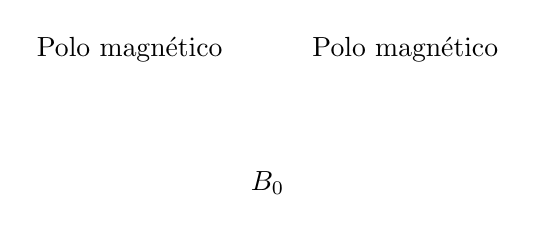
\begin{tikzpicture}

% Dibuja los polos magnéticos


% Etiqueta los polos
\node at (-1.75,1.2) {Polo magnético};
\node at (1.75,1.2) {Polo magnético};

% Dibuja el campo magnético
%\draw[->, thick] (-1.5,0.5) -- (1.5,0.5) node[midway, above] {Campo magnético \text{=} 0};

% Etiqueta B₀
\node at (0,-0.5) {$B_0$};

\end{tikzpicture}
\label{fig:marginfig2}
\end{marginfigure}

\begin{marginfigure}
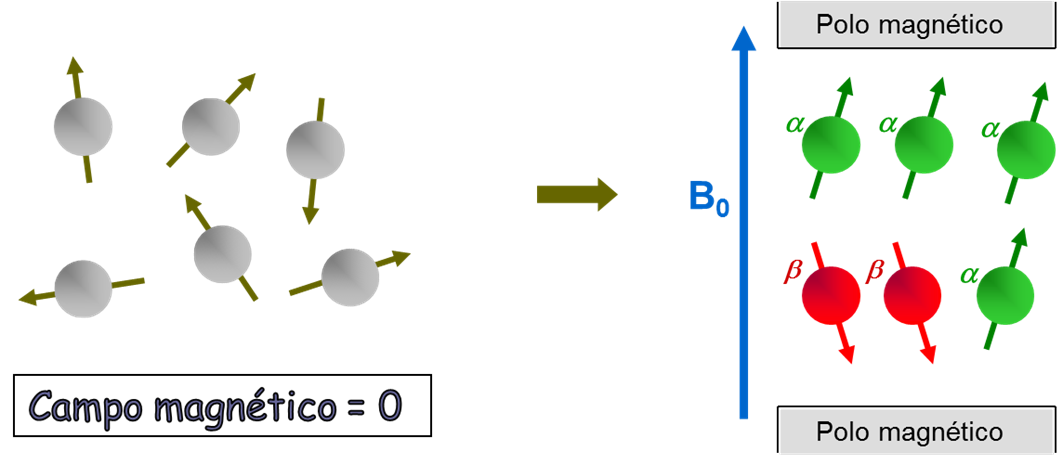
\includegraphics{Introduction/image.png}
\caption{\url{https://radiodiagnosticando.com/2016/06/13/rm-introduccion-a-conceptos-basicos-definicion-de-spin/}}
\label{fig:marginfig}
\end{marginfigure}

A continuación, como se muestra en la Figura~\ref{fig:marginfig} se emite un pulso de radiofrecuencia (RF) con una frecuencia específica (frecuencia de Larmor), lo que provoca que los protones absorban energía y cambien su alineación. Cuando cesa la excitación, los protones regresan a su estado de equilibrio, emitiendo señales electromagnéticas que son captadas por las antenas del equipo de RM [22]. Estas señales son procesadas mediante algoritmos de reconstrucción para generar imágenes en dos o tres dimensiones, que pueden ser visualizadas por el radiólogo en un monitor de computadora. La información obtenida en las imágenes de RM se basa en la distribución espacial de los protones en los tejidos, así como en sus propiedades magnéticas y de relajación, lo que permite obtener información detallada sobre la anatomía y fisiología del cuerpo humano [23].\cite{DBLP:conf/icann/2006-1}

\section{Objetivos de la Investigación} \label{sec:objetivos}
El objetivo principal de este trabajo es desarrollar un sistema de inteligencia artificial basado en redes neuronales convolucionales (CNNs) para la clasificación y segmentación automatizada de imágenes de resonancia magnética (RM) en pacientes oncológicos. Para ello, se plantean los siguientes objetivos específicos:
\begin{enumerate}
    \item Recopilar y preprocesar un conjunto de datos de imágenes de RM de pacientes oncológicos, incluyendo imágenes de tumores y tejidos sanos.
    \item Implementar un modelo de CNN para la clasificación de imágenes de RM en tejidos sanos y patológicos, evaluando su rendimiento en términos de precisión, sensibilidad y especificidad.
    \item Desarrollar un modelo de CNN para la segmentación de tumores en imágenes de RM, evaluando su capacidad para delimitar con precisión las regiones de interés.
    \item Integrar los modelos de clasificación y segmentación en una interfaz de usuario interactiva que permita la visualización y análisis de los resultados.
    \item Validar los modelos de IA en un conjunto de datos independiente, comparando sus resultados con los de especialistas humanos en radiología.
\end{enumerate}

\section{Estructura del Trabajo Fin de Grado} \label{sec:estructura}
El presente trabajo se estructura en cinco capítulos, cada uno de los cuales aborda aspectos específicos del desarrollo del sistema de inteligencia artificial para la clasificación y segmentación de imágenes de resonancia magnética en pacientes oncológicos. A continuación, se describen los contenidos de cada capítulo: 
\begin{enumerate}
    \item \textbf{Introducción:} En este capítulo se presenta una introducción general a la inteligencia artificial y su aplicación en medicina, así como los principios de las imágenes médicas y la resonancia magnética. Se describen los objetivos de la investigación y la estructura de la tesis.
    \item \textbf{Estado del Arte:} Se abordan los fundamentos teóricos de la inteligencia artificial, el aprendizaje profundo y las redes neuronales convolucionales, así como los principios de las imágenes de resonancia magnética y su aplicación en el diagnóstico y tratamiento de enfermedades.
    \item \textbf{Metodología:} Se describe la metodología utilizada en el desarrollo del sistema de inteligencia artificial, incluyendo la recopilación y preprocesamiento de datos, la implementación de modelos de CNN para clasificación y segmentación, y la evaluación de los resultados.
    \item \textbf{Resultados:} Se presentan los resultados obtenidos en la implementación de los modelos de CNN para la clasificación y segmentación de imágenes de resonancia magnética, así como su validación en un conjunto de datos independiente.
    \item \textbf{Conclusiones y Trabajo Futuro:} Se presentan las conclusiones del trabajo realizado, así como las limitaciones y posibles mejoras para futuras investigaciones en el campo de la inteligencia artificial aplicada a la medicina.
\end{enumerate}    